\documentclass{article}

\author{Pedro Henrique Limeira da Cruz}
\title{ET520 - Conversão de Energia}

\usepackage[margin=0.8in]{geometry}
\usepackage{indentfirst}
\usepackage{fancyhdr}
\usepackage{tcolorbox} 
\usepackage{graphicx}
\usepackage{amsmath}
\usepackage{amssymb}
\usepackage{enumitem}
\usepackage{tabularx} % in the preamble
\usepackage{wrapfig}

% Create a Todo list
\newlist{todolist}{itemize}{2}
\setlist[todolist]{label=$\square$}

\newcolumntype{Y}{>{\centering\arraybackslash}X}

% Create a new command to be used in the align environment in multiple line equations do only the last equation is numbered  
\newcommand{\n}{\nonumber \\ }
\makeatletter
\let\inserttitle\@title
\makeatother
% Set the style of the page 
\pagestyle{fancy}
\fancyhf{}
\rhead{Pedro Henrique L. da Cruz}
\lhead{\inserttitle}
\rfoot{Page \thepage}

\usepackage{hyperref}
\hypersetup{
    colorlinks=true,
    linkcolor=black,
    filecolor=magenta,
    urlcolor=cyan,
}

% Begin the Document 
\begin{document}

\maketitle
\thispagestyle{empty}

% Add the image inside a figure in as the first page
% \begin{figure}[h]
%     \begin{center}
%         
\includegraphics[scale = 0.15]{/Users/pedrocruz/Documents/UNICAMP/ES101/ES101 - Robotic Arm/img/unicamp.png}
%     \end{center}
% \end{figure}

% Change to the Next page 
\newpage
\tableofcontents
\newpage

\section{Introdução}
De modo geral, existem quatro princípios de como os campos magnéticos são utilizados em máquinas elétricas, sendo eles:

\begin{itemize}
    \item \textbf{Produção de Campo - Simples}: Um fio conduzindo uma corrente elétrica produz um campo magnético sem sua vizinhança.
    \item \textbf{Ação Transformador}: Um campo magnético variável no tempo induzirá uma tensão em uma bobina se este campo passar através de dela.
    \item \textbf{Ação Motor}: Um fio conduzindo corrente elétrica, na presença de um campo magnético, tem uma força induzida sobre ele.
    \item \textbf{Ação Gerador}: Um fio movendo-se na presença de um campo magnético tem uma tensão induzida nele.
\end{itemize}

Para que possamos entender melhor sobre cada um dos princípios acima, precisamos primeiro sermos capazes de representar as diferentes topologias que estão envolvidas e simplificar as contas, através da criação de modelos. 

Como temos muita familiarização com os modelos criados para circuitos, iremos criar um paralelo entre circuitos elétricos e o que chamaremos de \emph{circuitos magnéticos}.


\section{Circuitos Magnéticos}
\subsection{Produção de Campo Magnético}
\subsubsection{Relação $i-H$}

Antes de vermos a representação e simbologias utilizadas para os modelos de circuitos magnéticos, precisamos primeiro entender como eles são gerados.


\begin{wrapfigure}{r}{0.40\textwidth}
    \vspace{-25px}
    \centering
    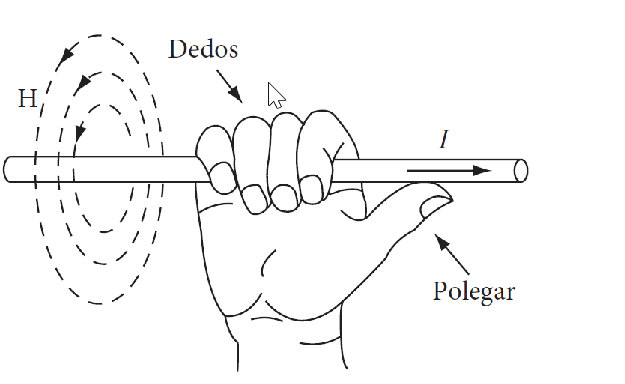
\includegraphics[width=0.3\textwidth]{imgs/2023-08-15 10_18_18-1_CIRCUITOS_MAG.pdf - ET520 - Princípios de Conversão de Energia - Visual Studio.png}
    \caption{Regra da Mão Direita}
    \label{img:regra_da_mao_direita}
\end{wrapfigure}

Como dito na listagem dos princípios magnéticos (no começo do capítulo), um \textbf{campo é gerado sempre que uma corrente passa em um condutor}, onde a direção de tal campo pode ser determinado pela direção da corrente (utilizando da regra da mão direita, como mostrado na imagem \ref{img:regra_da_mao_direita}).

Partindo do axioma acima, conseguimos modelar matematicamente a relação entre campo e corrente, mis especificamente a relação entre a \textbf{Intensidade de Campo Magnético $H$} e corrente:
\begin{align}
    \oint \vec H \cdot \vec{dl} = i_{net}
\end{align}

Onde:
\begin{itemize}
    \item $\vec H$: Representa o vetor Intensidade de Campo.
    \item $\vec{dl}$: Representa o vetor comprimento do elemento infinitesimal de fio sob análise.
    \item $i_{net}$: Representa a corrente resultante, utilizada se há mais de um frio conduzindo corrente. 
\end{itemize}

\newpage

Desenvolvendo essa integral de linha, para um caso simplificado onde a linha é representada por um circulo de raio $r$, temos:

\begin{wrapfigure}[3]{l}{0.40\textwidth}
    \centering
    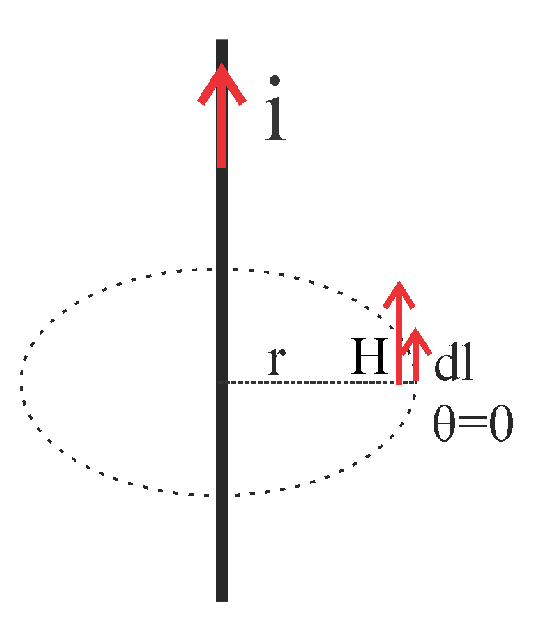
\includegraphics[width=0.20\textwidth]{imgs/2023-08-15 11_04_26-1_CIRCUITOS_MAG.pdf - ET520 - Princípios de Conversão de Energia - Visual Studio.png}
    \caption{Calculo - Intensidade $H$}
\end{wrapfigure}
$ $
\begin{align}
    &\oint \vec H \cdot \vec{dl} = i \n
    &\oint  H dl \cos \theta = i , \ \  \vec H \parallel \vec{dl} \therefore \theta = 0 \n
    &\oint  H dl = i \n 
    &H \oint  dl = i \n 
    &H 2 \pi r = i \n 
    &H = \frac{i}{2 \pi r }
\end{align}

\vspace{30px}
$ $
Para o caso específico de espiras, podemos ainda relacionar a intensidade $H$ com a corrente e a quantidade de voltas dada:

\begin{align}
    \oint \vec H \cdot \vec{dl} = Ni \n
    H l = Ni
    \label{eq:intensidade_espiras}
\end{align}

Onde o $l$ representa o chamado \textbf{Caminho Médio} da área na qual foi enrolada a espira, isso é, no caso de um toroid de raio $r$, no qual foram feitas $N$ voltas de fio, o $l$ é dado por $l=2\pi r$.

É importante ter em mente que a intensidade $H$ representa o \textbf{esforço} que a corrente precisa fazer para estabelecer um campo magnético.

\subsubsection{Relação $H-B$}
A intensidade $H$ do campo produz uma densidade de fluxo $B$ em todos os pontos que existe, dada por: 
\begin{align}
    B = \mu H
\end{align}

Onde $\mu$ representa a \textbf{Permeabilidade Magnética}, referente ao material no qual a intensidade está gerando a densidade magnética. Normalmente, entretanto, essa permeabilidade tem valores muito extremos (tanto para mais, como no caso de materiais ferro-magnéticos, quanto para menos, como no caso do vácuo $\approx$ ar), por isso nós usualmente utilizamos:

\begin{align}
    B = \mu_{r} \mu_{Vac} H
\end{align}

Onde $\mu{r} = \mu{relative}$ é a permeabilidade magnética do material relativo (i.e divide) a permeabilidade do vácuo $\mu_{0} = \mu_{vac} = 4\pi 10^{-7}$. Como consequência, para a análise de densidade no vácuo, ar, isloantes ou condutores elétricos (como cobre ou alumínio) o $\mu \approx \mu_0 \therefore \mu_r = 1$.

Além disso, é interessante analisar a relação entre permeabilidade ($\mu$), intensidade ($H$) e densidade ($B$):

\begin{align*}
    B = \mu H \Rightarrow \begin{cases}
        B = const & \downarrow \mu \therefore \uparrow H \\ 
        H = const & \downarrow \mu \therefore \downarrow B
    \end{cases}
\end{align*}

\subsubsection{Fluxo Magnético}

De uma forma geral, somos capazes de calcular o \textbf{fluxo magnético} $\Phi$, passando por um core magnético no cenário onde não há leakage \footnote{leakage é o fenômeno onde parte do fluxo de campo passar por fora do core e é perdido} pela equação:
\begin{align}
    \Phi = B A_C
\end{align}

Onde $A_C$ representa a área, constante, do core ferro-magnético.


\subsection{Circuito Magnético Equivalente}
Agora que temos as equações básicas para calcularmos os principais elementos magnéticos, iremos fazer o paralelo com os circuitos elétricos, começando pela  \textbf{Força Magneto Motriz} $\mathcal{F}$, que faz o paralelo com a tensão em circuitos convencionais.
\begin{align}
    \mathcal{F} = Hl = \underbrace{Ni}_{Espiras}
\end{align}

Onde, para o caso de espiras, o $N$ representa a quantidade de voltas, como mostrado na equação \ref{eq:intensidade_espiras}.

A partir disso, podemos fazer, então, o paralelo da lei de Ohm para circuitos magnéticos, sendo ele:
\begin{align}
    \Phi &= B A \n 
         &= (\mu H) A \n 
         &= \frac{\mu N i}{l} A \Leftarrow Hl = Ni \therefore H = Ni/l \n
         &= \frac{\mu N i}{l} A \frac{1/(\mu A)}{1/(\mu A)} \n
         &= \frac{N i}{l/(\mu A)} \n
         &= \frac{\mathcal{F}}{\mathcal{R}} \ \ { \atop{\rightarrow \ Relut\hat{a}ncia}}
\end{align}


A partir desses conceitos, nós somos capazes de resolver problemas relativamente complexos, ao representarmos ele como um circuito magnético, com uma força magneto motriz (referenciando uma tenção), relutâncias (referenciando resistências, sendo que cada materias/estágio do circuito magnético possui um) e um fluxo magnético (que tem como contrapartida a corrente elétrica), como podemos ver pela image \ref{img:circuito_equivalente}.
\begin{figure}[h]
    \centering
    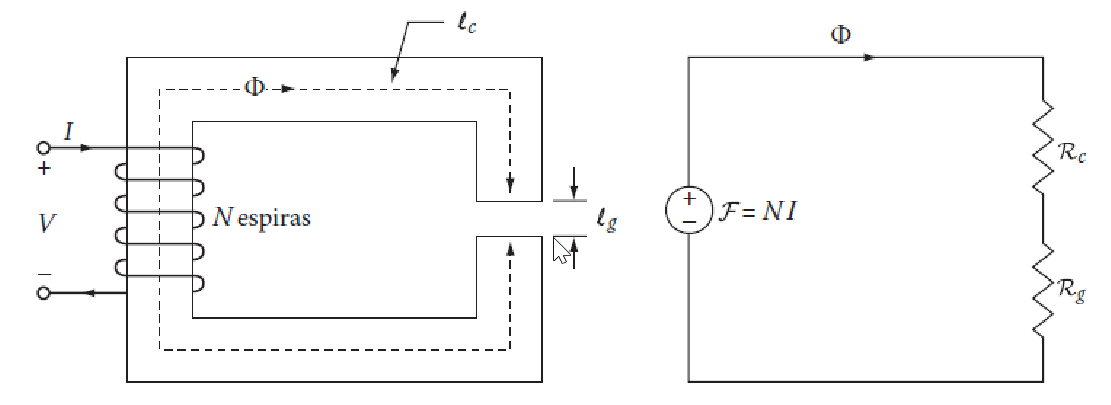
\includegraphics[width=0.7\textwidth]{imgs/circuito_equivalente.png}
    \caption{Circuito Equivalente}
    \label{img:circuito_equivalente}
\end{figure}

\newpage
\subsubsection{Considerações Sobre Circuitos Magnéticos}
Os calculos e as fórmulas que foram descritas anteriormente, são boas aproximações que podemos fazer quando estamos trabalhando com problemas de engenharia. Elas aindasão, entretanto, aproximações, logo as hipóteses que são levadas em consideração precisam ser mantidas em mente, sendo as principais:

\begin{itemize}
    \item Não consideração do \textbf{Fluxo de disperção}, i.e fluxos que se originam na expira mas que não ocorrem atavéz do core, mas sim se disperção no meio (como ar).
    \item Aproximação do \textbf{Caminho Médio}: O caminho que consideramos que o fluxo percorre $l$, que é utilizado no calculo da intensidade $H$ (eq \ref{eq:intensidade_espiras}) é denominado de caminho médio, mas na realidade há diferentes caminhos percorrido pelo campo.
    \item \textbf{Saturação Magnética}: Ocorre quando não é possível aumentar a intensidade do fluxo magnético, mesmo com o aumento da corrente.
    \item \textbf{Espraiamento}: Em seções de entre-ferro, o fluxo magnético não ocorre em linhas retas, mas sim ocorre um alongamento do caminho percorrido, aproximando-se de uma esfera alongada.
\end{itemize}

\subsection{Fluxo Concatenado - Lei de Faraday-Lenz}
Na introdução da matéria, vimos que existem $4$ principais Fenômenos, sendo eles a produção de capo, a ação trasnformador, a açao Motor e por fim a ação gerador. Iremos agora, explicar o fenômeno de geração de tensão a partir da presença de uma espira em um campo que varia com o tempo.

De forma matemática, isso é representado por:
\begin{align}
    e &= -N \frac{d \Phi}{dt} \n
      &= -\frac{d\lambda}{dt}, \ \ \lambda = N\Phi \rightarrow \ Fluxo\ Concatenado
      \label{eq:fluxo_concat}
\end{align}

Onde o fluxo concatenado $\lambda$, como o nome indica, é a "concatenação" (ou associação/soma/junção) dos campos gerados em cada volta da espira.

O que a equação \ref{eq:fluxo_concat} representa é que, se uma expira, com $n$ voltas, está na presença de um campo variante no tempo, uma tensão $e$ é induzida nos terminais de tal rolamento.

Isso, entretanto, juntamente do fenômeno de produção de campo (que diz que todo indutor que esteja conduzindo gera um campo magnético) resulta no que chamamos de \textbf{Lei de Lenz}, isto é, ocorre a geração de um campo magnético de fluxo de oposiçaõ, como ilustrado pela imagem abaixo.
\begin{figure}[h]
    \centering
    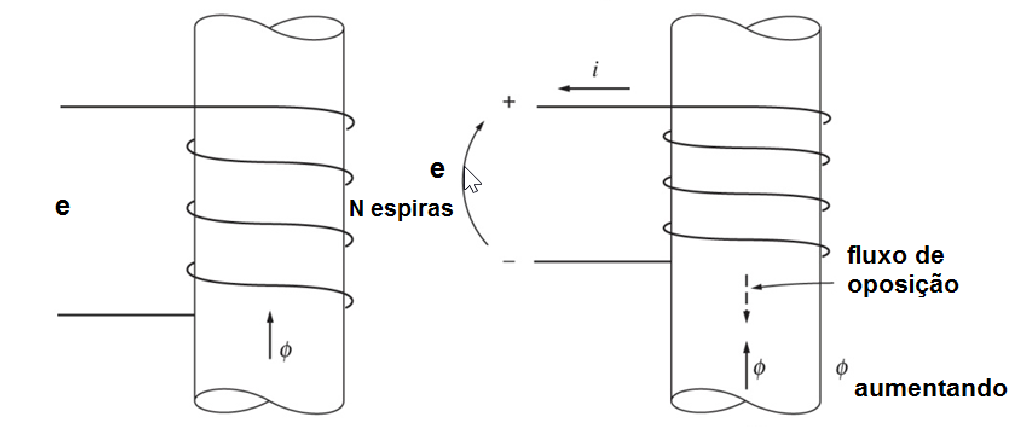
\includegraphics[width=.6\textwidth]{imgs/leinz.png}
    \caption{Lei de Lenz}
    \label{fig:leinz}
\end{figure}

\newpage
\subsection{Indutância}
Em um cenário sem a ocorrência de saturação magnética, podemos definir a indutância como sendo a relação entre a corrente de alimentação e o fluzo concatenado, dado por:
\begin{align}
    L = \frac{\lambda}{i}
    \label{eq:indutancia}
\end{align}

Fisicamente, a indutância está relacionada a quantidade de energia armazenada na forma de campo magético, i.e quanto maior a indutância $L$ para uma mesma corrente, maior a quantidade de energia e maior o fluxo magnético.

\subsection{Indutância Mútua}
Existem topologias, entretanto, que ocorre o chamádo \textbf{indutãncia mútua}. Esse fenômeno ocorre quando um circuito magnético apresenta dois rolamentos, resultando em uma "contaminação" de um rolamento no outro, isso é, a indutância resultante em cada uma das espiras é composta pela própria indutância (chamada de indutância própria), juntamente com a "indutância mútua" (efeito da outra).

\begin{figure}[h]
    \centering
    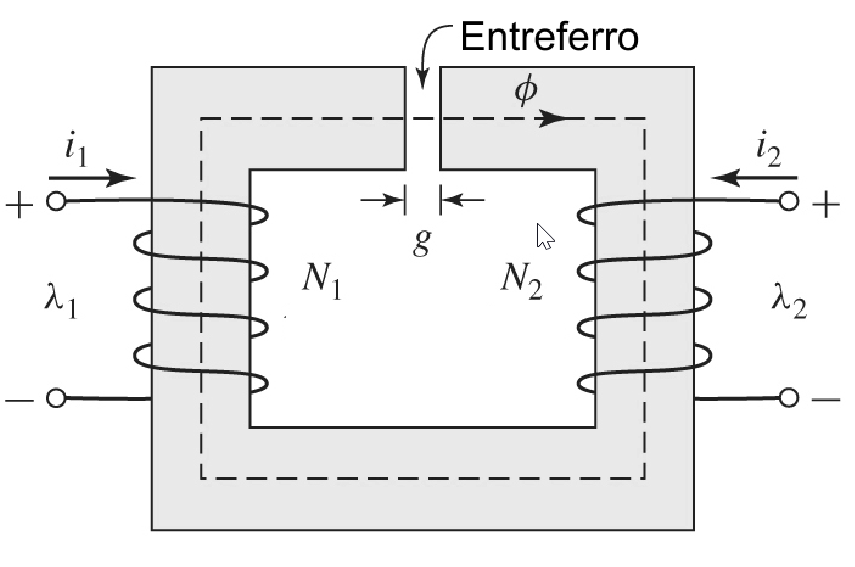
\includegraphics[width=.6\textwidth]{imgs/mutua.png}
    \caption{Circuito com Indutância Mutua}
    \label{fig:mutua}
\end{figure}

Matematicamente, isso é expresso da seguinte forma:

\begin{align}
    L_{11} = N_1^2 \frac{\mu_0 A_c}{g}, L_{12} = N_1N_2\frac{\mu_0 A_c}{g} \\ 
    \underbrace{L_{22} = N_2^2 \frac{\mu_0 A_c}{g}}_{Indut\hat{a}ncia \ Pr\acute{o}pria}, \underbrace{L_{21} = N_1N_2\frac{\mu_0 A_c}{g}}_{Indut\hat{a}ncia \ M\acute{u}tua}
\end{align}

Onde o fluxo concatenado resultante seria dado por:
\begin{align}
    \lambda_1 = L_{11}i_1 + L_{12}i_2 \n
    \lambda_2 = L_{22}i_2 + L_{21}i_1
    \label{eq:indu_mut}
\end{align}

As equações acima são válidas somente para esse caso onde possui entreferroe é simétrico. Nos casos gerais, entretanto, temos que usar ou a equação \ref{eq:indu_mut} (se estivermos fazendo literalmente) ou podemos ainda usar o princípio da superposição:
\begin{enumerate}
    \item Aplicar Uma corrente de $1A$ em um dos lados - Deixando o outro lado sem nada, aplicar uma corrente em um dos lados e achar qual o fluxo que passa em cada espira.
    \item Achar Indutância - A partir do fluxo que passa por cada espira, e tendo $i = 1A$, podemos utilizar a definição de indutância da equação \ref{eq:indutancia}, juntamente com a equação \ref{eq:fluxo_concat} para calcular a indutância própria (utilizando o fluxo que passa na própria espira que estamos aplicando a corrente) e a indutância mútua (utilizando o fluxo e o número de voltas da espira vazia):
    \begin{align}
        L = \frac{1}{i} N \Phi
    \end{align}

    \item Repetir esse procedimento, mas agora substituindo em qual espira a corrente de $1A$ é aplicada, onde acharemos então a indutância mútua da outra espira e acharemos a outra indutância mútua (em geral as indutâncias mútuas vão ser bem próximas).
\end{enumerate}

\subsection{Energia Armazenada}
De forma geral, circuitos magnéticos também podem ser usados para armazenar energia na forma de energia magnética. Para tais casos, sendo os circuitos contendo somente um enrolamento, somos capazes de calcular a potência armazenada como sendo:
\begin{align}
W(\lambda) = \frac{1}{2L}\lambda^2, \ \ \ \ W(i) = \frac{1}{2}Li^2
\end{align}

\subsection{Propriedades dos Materiais Magnéticos}
\subsubsection{Ciclo de Histerese}
Antes de definir o que seria o ciclo de Histerese, é importante entendermos o comportameno do material quando submetido a um campo magnético. 

Podemos modelar um material como sendo uma junção de várias pequenas regiões, denominadas de \textbf{Domínios Magnéticos}, onde dentro de cada um desses domínios, os átomos (que podemos pensar como flechas) estão alinhadas em uma direção, cada um agindo como um pequeno imã.

Quando um material está desmagnetizado, cada um desses domínios estáo orientados aleatoriamente de forma que os campos gerados se cancelem. Na presença de um $H$ (intensidade magnética), entretanto, todos esse domínios tendem a se alinhar com a direção de tal intensidade.

Em um cenário perfeito, assim que tirássemos o material da presença da intensidade magnética $H$, todos os domínios iriam voltar para sua posição de origem e o materia iria voltar a não estar magnetizado. 

Na realidade, entretanto, isso não ocorre e, após a presença de uma intensidade magnética $H$, nem todos os domínios magnéticos volta a sua posição original, resultando em uma \textbf{Magnetização Residual}. 

Tal magnetização residual resulta em uma curva de magnetização que náo é circular (\emph{i.e} ele não volta de onde paprtiu), o que chamamos de \textbf{Histerese}.

\subsubsection{Saturação}
\subsubsection{Corrente de Foucault}

\newpage
\section{Transformadores}
\subsection{Introdução}
Iremos agora estudar sobre os transformadores. Os transformadores são extremamente importantes em sistemas de conversão de energia, mesmo ele não sendo um (ele converte energia elétrica para elétrica, e não para outro tipo de energia).  Sua importância, entrentanto, é inegável, principalemnte em sistemas de conversão e distribuição de energia (como por exemplo transmitir energia que foi gerada em uma hidro-elétrica para as casa, ...).

Os transformadores são construídos basicamente com dois (ou mais) enrolamentos acomplados por um fluxo magnético em comum, onde na maioria das vezes, para aumentar a eficiência, está presente um núcleo de material ferro-magnético (como vimos nos capítulos passados). O enrolamento conectado a fonte de corrente alternada é denominado de \textbf{Primário}, e o conectado ao load é conhecido como \textbf{Secundário}. 

Seu princípio de funcionamento é:  Uma corrente alternada é aplicada ao primário, gerando assim um campo magnético variante no tempo. Como temos que o primário e o secundário estão acomplados sob o mesmo campo, o secundário está na presença de um campo variante e por conseguinte desenvolve uma tensão, também alternada.

\subsection{Modelagem}
\subsubsection{Transformador Ideal}
O primeiro passo para entendermos melhor o funcionamento de um transformador é pensar da forma mais simples possível, através de um cenário ideal. 

Um transformador Ideal, com dois enrolamentos (primário com $N1$ espiras e o secundário com $N2$ espiras), possui as seguintes simplficiações e a seguinte modelagem:

\begin{figure}[h]
    \centering
    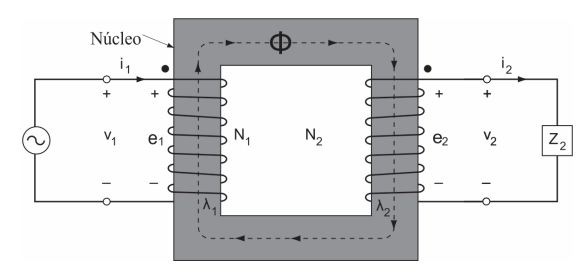
\includegraphics[width=0.5\textwidth]{imgs/transformador_ideal.png}
    \caption{Transformador Ideal}
    \label{fig:transformador_ideal}
\end{figure}

\vspace{10px}
\begin{minipage}{0.5\textwidth}
\begin{itemize}
    \item  Resistência dos enrolamentos é nula
    \item Todo fluxo é concatenado pelo núcleo
    \item Não há perdas no núcleo
    \item A permeabilidade do núcelo $\mu$ muito alta, corrente de excitação desprezível.
\end{itemize}
\end{minipage}
\begin{minipage}{0.5\textwidth}
    \begin{align}
        \frac{N1}{N2} &= \frac{v_1}{v_2} = a \label{eq:tens_transformador}\\ 
        \frac{i_1}{i_2} &= \frac{1}{a}
    \end{align}
\end{minipage}
\vspace{10px}

Onde podemos ver que as tensões são diretmanete proporcionais à $a$, que chamamos de \textbf{Relação de Transformação}, já a corrente é inversamente proporcional.

Podemos, ainda, verificar que, através da relação de transformação, podemos \textbf{Refletir Impedâncias} de um enrolamento para outro, isso é, se há uma impedância no enrolamento 1, mas isso torna a análise mais difícil, podemos "refletir" tal impedância do enrolamento um para o dois, retirando-a do enrolamento 1 (ou vice-versa), através da seguinte relação:
\begin{align}
    Primario&\rightarrow Secundario: z_1 \rightarrow (1/a^2)z_1\\
    Secundario&\rightarrow Primario: z_2 \rightarrow a^2z_2
\end{align}

\subsubsection{Transformador Real}
Até o momento, nós temos um modelo simples de entender e de ser analisado (o transformador ideal) mas para certas aplicações ele não é suficiente para caracterizarmos e modelarmos um transformador.

A fim de modelarmos de uma maneira mais verossímil, nós podemos acrescentar ao modelo da imagem \ref{fig:transformador_ideal} os seguintes elementos:

\begin{figure}[h]
    \centering
    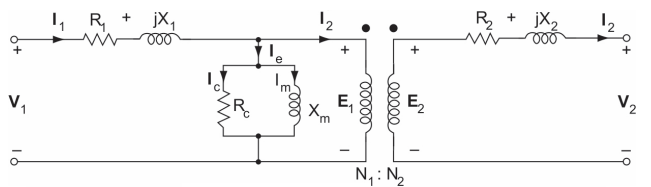
\includegraphics[width=0.5\textwidth]{imgs/transformador_real.png}
    \caption{Modelo de Transformador Real}
    \label{fig:trasnformador_real}
\end{figure}

\begin{enumerate}
    \item \textbf{Resistências dos Enrolamentos}: Para representarmos a ressitência elétrica dos fios que compoem os enrolamentos nós podemos adicionar $R_1$ e $R_2$, nos terminais de entrada e saída dos primário e do secundário, respectivamente.
    \item \textbf{Fluxo Disperso}: Para representarmos o fluxo que acaba sendo disperso, e não sendo direcionado pelo núcleo, podemos colocar duas reatâncias $X_{l1}$ e $X_{l2}$, onde:
    \begin{align}
        L_{l1} = \frac{N_1 \phi_1}{i_1} \rightarrow X_{l1} = 2\pi f L_{l1} \\
        L_{l2} = \frac{N_2 \phi_2}{i_2} \rightarrow X_{l2} = 2\pi f L_{l2}
    \end{align}

    \item \textbf{Corrente de Excitação}: A corrente de excitação representa a corrente mínima necessária para suprir as perdas do núcelo e gerar um campo magnético. Para sua representação, nós botamos, em paralelo com a representação do enrolamento um, uma reatância (chamada de \emph{indutância de magnetização}):
    \begin{align}
        X_m = 2\pi fL_M
    \end{align}

    \item \textbf{Perdas no Núcelo}: Para representar as perdas no núcelo, nós botamos uma resistência (em paralelo com a indutância  de magnetização) uma resistência $R_C$
\end{enumerate}

\newpage
\subsubsection{Ensaios de Determinação de Parâmetros}
A fim de determinarmos quais são os parâmetros que foram citados anteriormente, é necessário a realização de uma série de ensaios.

\begin{itemize}
    \item \textbf{Ensaio CC}: Utilizado para medir as resistÊncias dos enrolamentos. O Ensaio é realizado através da aplicação de uma baixa tensão $CC$ nso enrolamentos, e mendindo sua corrente. Através da relação de Ohm conseguimos calcular as resistências.
    \item \textbf{Ensaio de Circuito Aberto}: Utilizado para determinar a indutância de Magnetização $X_m$. O ensaio consistem em aplicar uma tensão senoidal em um enrolamento, com o outro em aberto. Medindo, então, a tensão sendo aplicada ($V_{ca}$), a corrente do primário ($I_{ca}$) e a potência ($P_a$), como ilustrado abaixo, somos capazes de achar $X_m$:
    
    \begin{minipage}{0.5\textwidth}
        \centering
        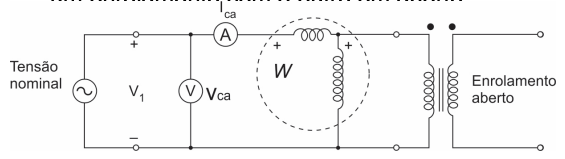
\includegraphics[width=\textwidth]{imgs/calculo_xm.png}
    \end{minipage}
    \begin{minipage}{0.5\textwidth}
        \begin{align}
            R_c = \frac{V_{ca}^2}{P_a}; |Z| = \frac{V_{ca}}{I_{ca}} \n 
            X_m = \frac{1}{\sqrt{\left(\frac{1}{|Z|}\right)^2 - \left(\frac{1}{R_c}\right)^2}}
        \end{align}
    \end{minipage}

    \item \textbf{Ensaio de Curto Circuito}: Esse ensaio é utilizado para encontrarmos as reatâncias $X_{l1}$ e $X_{l2}$ (que representam o fluxo de dispersão). Nesse ensaio é aplicado uma tensão senoidal reduzida no enrolamento com o outro enrolamento em curto circuito. A tensão deve ser regulada até que flua uma corrente nominal \footnote{Como temos uma corrente nominal, temos que a potência gerada também é nominal (normalmente dada pelo data-sheet e enunciado do problema)} no lado do curto circuito.

    \begin{minipage}{0.5\textwidth}
        \centering
        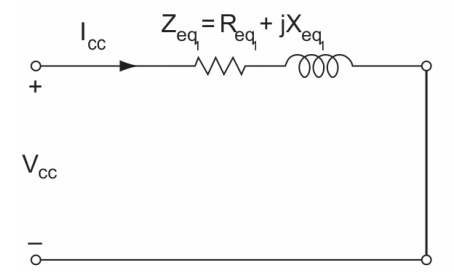
\includegraphics[width=0.7\textwidth]{imgs/ensaio_curto.png}
    \end{minipage}
    \begin{minipage}{0.5\textwidth}
        \begin{align}
            Z_{cc} &= \frac{V_{cc}}{I_{cc}}\n
            R_{eq} &= \frac{P_{cc}}{I^2_{cc}}\n
            X_{eq} &= X_{l1} + X'_{l2} = \sqrt{Z^2_{cc} - R^2_{cc}}, \n X_{l1} &= X'_{l2}
        \end{align}
    \end{minipage}

\end{itemize}

\newpage
\subsection{Regulação de Tensão}
Até o momento, nós vimos que existe uma relação entre a tensão do primário e tensão do secundário para o caso ideal (dada pela equação \ref{eq:tens_transformador}), onde não há perdas e não há um carregamento no secundário.

Ao conectarmos uma carga ao secundário, sua tensão não será mais $V_S = V_1/a$, pois haverá uma querda de tensão na impedância do transformador (pois haverá a presença de uma corrente). Definimos então que a \textbf{Regulação de Tensão} ($VR$) é a relação entre a tensão do secundário em vazio $|V_{2NL}|$(\emph{i.e} sem carga), com a tensão plena com carga $|V_{2N}|$:
\begin{align}
    VR = \frac{|V_{2NL}| - |V_{2N}|}{|V_{2N}|}\times 100%
\end{align}

Onde a tensão no secundário depende da carga:
\begin{align}
    \frac{V_1}{a} = V_2 + \underbrace{R_{eq2}I_2 + jX_{eq2}I_2}_{Perda \ da \ carga}
\end{align}

Onde a resistência (que pode ser indutiva, capacitiva, resistiva ou uma combinação de todos esses) $R_{eq} + jX_{eq}$ é a impedância total "enxergada" do segundo enrolamento. Como tal impedância pode ser de diferentes naturezas, o valor do $VR$ vai se comportar de uma forma diferente para cada:

\begin{table}[h]
    \centering
    \begin{tabular}{l c c c}
        \textbf{Tipo de Carga} & \textbf{Fator de Potência} & \textbf{Regulação de Tensão (VR)} & \textbf{Diagrama} \\ 
        Carga Indutiva & FP -  &  VR + & 
        
        \begin{minipage}{0.3\textwidth}
            \centering
            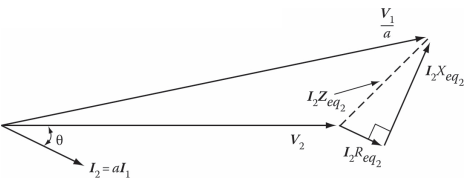
\includegraphics[width=\textwidth]{imgs/vr_indutivo.png}
        \end{minipage} 
        
        \\
        Carga Capacitiva & FP +  &  VR - &  \begin{minipage}{0.3\textwidth}
            \centering
            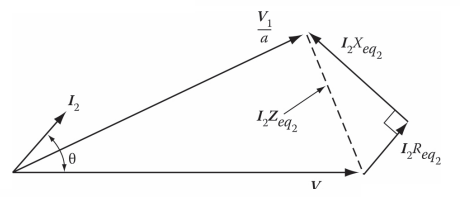
\includegraphics[width=\textwidth]{imgs/vr_capacitivo.png}
        \end{minipage}\\
        Carga Resistiva & FP = 1  &  VR $\rightarrow$ min & \begin{minipage}{0.3\textwidth}
            \centering
            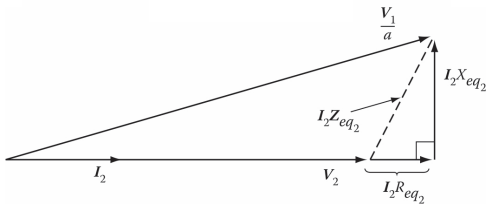
\includegraphics[width=\textwidth]{imgs/vr_resistivo.png}
        \end{minipage}\\
    \end{tabular}
    \caption{Influência da Carga no VR}
    \label{tab:vr_carga}
\end{table}

Onde é importante relembrar o que é o \textbf{Fator de Potência} ($FP$). O fator de potência é a relação entre a \textbf{Potência Ativa} (aquela que podemos converter para outro tipo de energia, como mecânica, calor, etc), a \textbf{Potência Reativa}, que não podemos transformar em nada e é utilizada para a criação do campo magnético, logo é importante para equipamentos que funcionam por indução, como motores, transformadores, etc e a \textbf{Potência Aparente}, que representa a potência total e é a soma da potência ativa e reativa.

O $FP$ é dado por:

\begin{minipage}{0.5\textwidth}
    \centering
    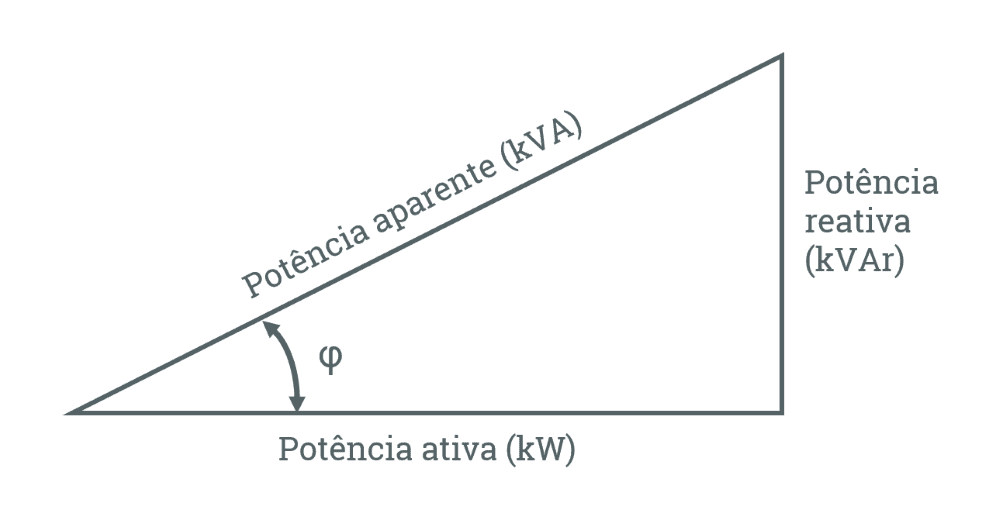
\includegraphics[width=\textwidth]{imgs/triangulo-de-potencias-usado-em-fator-de-potencia.png}
\end{minipage}
\begin{minipage}{0.5\textwidth}
    \begin{align}
        FP = \cos{(\phi)} &= \frac{P. \ Ativa}{P. \ Aparente}
    \end{align}
\end{minipage}

\subsection{Rendimento}
De forma gera, quando estamos falando de rendimento de qualquer máquina/processo, nós falamos da saída/entrada. 

No caso dos transformadores, temos que o rendimento $\eta$ é dado por Potência de saída / potência de entrada, resultando em:

\begin{align}
    \eta &= \frac{Pot. \ Saida}{Pot. \ Entrada} \n 
         &= \frac{P_{out}}{P_{out} + P_{Losses}} \n 
         &= \frac{V_2 I_s \cos \theta_2}{V_2 I_s \cos \theta_2 + {I_2^2 R_{eq}}_2}
\end{align}

\subsection{Autotransformador}
O Autotransformador é uma configuração especial em que um enrolamento comum ao primário e ao secundário é montado sobre um núcleo do transformador. Isso significa que \textbf{Não Há separação Fisica entre um enrolamento e outro}, o que é uma das principais vantages dos transformadores tradicionais. 

\begin{minipage}{0.5\textwidth}
   \centering
   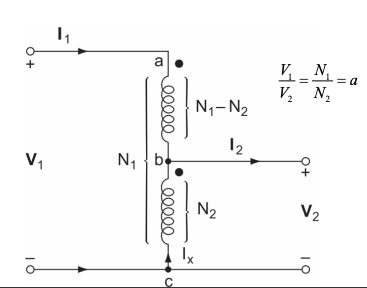
\includegraphics[width=0.6\textwidth]{imgs/auto_transformador.png}
\end{minipage}
\begin{minipage}{0.5\textwidth}
\vspace{-25px}
As principais vantagens desse tipo de transformador é:
\begin{itemize}
    \item Mais barator
    \item Menos disperção
\end{itemize}
\end{minipage}

$\\$


\end{document}